\documentclass[12pt]{article}

% Packages
\usepackage[utf8]{inputenc}
\usepackage[T1]{fontenc}
\usepackage[margin=1in]{geometry}
\usepackage{amsmath,amssymb}
\usepackage{graphicx}
\usepackage{hyperref}
\usepackage{url}
\usepackage{booktabs}
\usepackage{enumitem}
\usepackage[numbers]{natbib}
\usepackage{authblk}
\usepackage{lineno}
\usepackage{subcaption}

% Graphics path
\graphicspath{{Figures/}}

\begin{document}

\title{OpenCell Design: An Open-Source Python Library for Construction, Energetic and Technoeconomic Modelling of Battery Cell Designs}

\author[1]{Nicholas Siemons\thanks{Corresponding author}}
\author[1]{Adrian Yao}
\affil[1]{Department of Materials Science and Engineering, Stanford University, Stanford, CA 94305, USA}

\maketitle

\begin{abstract}
The design and optimization of metal-ion battery cells requires the integration of material properties and cell architecture into a coherent modeling framework. We present OpenCell Design, an open-source Python library that provides a hierarchical, composable API for building virtual battery cells from individual components and materials. The software implements a physically intuitive modeling hierarchy spanning materials, formulations, electrodes, layups, electrode assemblies, encapsulations and complete cells. Users can construct cylindrical, prismatic, and pouch cell architectures using round or flat wound jelly rolls, stacked assemblies, or z-fold stacked assemblies. Four key features enable practical design workflows using OpenCell Design. First, a hierarchical update propagation system allows users to modify any parameter at any level of the cell hierarchy, with changes automatically propagating upward to update all dependent calculations. Second, a modular object-oriented architecture allows users to extend the library with custom components such as new materials, current collector geometries, and entirely new cell formats by subclassing the provided base classes. Third, a compact binary serialization format allows cell designs to be saved, shared, and version controlled. Fourth, interactive browser-based visualizations provide immediate visual feedback through cross-section views, capacity curves, and hierarchical cost and mass breakdowns.
\end{abstract}

\noindent\textbf{Keywords:} battery, cell design, open-source, Python, technoeconomic modeling

\vspace{1em}

\newpage

%% ============================================================================
\section{Introduction}
%% ============================================================================

The global transition to electrified transportation and grid-scale energy storage has placed increasing demands on energy storage technologies~\cite{chu2012opportunities,dunn2011electrical}. Metal-ion batteries have emerged as the dominant technology for applications ranging from portable electronics to electric vehicles and stationary storage~\cite{goodenough2013li,blomgren2017development}. In such applications, thermodynamic properties---such as specific and volumetric energy density---are critically important to their performance and to the progress of such technologies. Equally important are technoeconomic metrics---such as cost per unit energy stored---as these properties ultimately drive the adoption of energy storage technologies~\cite{nykvist2015rapidly,ziegler2021re}. Understanding the design and material drivers behind cell performance and cost is critical for further research, development and investment in metal-ion batteries.

Evaluating the drivers of performance and cost requires modeling of the cell at multiple scales. A single cell comprises dozens of interacting parameters and many individual components, spanning individual materials, electrode formulations, current collectors, separators, electrodes and encapsulations. Changes at the material level propagate through to cell-level performance and cost in complex ways, as do design choices associated with certain cell components. Furthermore, changes to the cell design may equally manifest at the cell level in important ways.

OpenCell Design is an open-source Python library that addresses this challenge by providing a hierarchical, composable API for building virtual battery cells from their individual components and materials. OpenCell Design calculates mass and cost at every level of the hierarchy, enabling direct assessment of economic viability alongside kinetic performance parameters.

%% ============================================================================
\section{Existing Software}
%% ============================================================================

Several software tools have been developed to support battery cell modeling, each addressing different aspects of the design challenge. PyBaMM~\cite{sulzer2021pybamm} is an open-source library for physics-based electrochemical simulation of batteries. It provides a flexible framework for constructing and solving models such as the Doyle--Fuller--Newman equations, enabling detailed analysis of ion transport, reaction kinetics, and thermal behavior during charge and discharge. PyBaMM excels at predicting dynamic cell behavior and has become widely adopted in the research community. However, its focus is on electrochemical phenomena rather than cell engineering: it does not model the geometric construction of cells from discrete components, nor does it calculate mass and cost breakdowns from the material level upward.

BatPaC~\cite{nelson2019batpac} and CAMS~\cite{cams2023}, developed by Argonne National Laboratory and the Faraday Institution respectively, take a complementary approach. They provide models that estimate the manufacturing cost and performance of battery packs and cells as a function of the cell design. However, both BatPaC and CAMS are implemented as Microsoft Excel workbooks, which limits extensibility and integration with programmatic workflows. A further limitation of these approaches is that they are unidirectional models---the outputs rely on a single set of parameter inputs, and bi-directional parameter setting is not possible.

Other tools exist for specific aspects of battery design, including electrode formulation calculators and capacity matching spreadsheets, but these typically address isolated aspects of cell design rather than the complete hierarchy from materials to cells. A gap remains for an open-source, programmatic and API-friendly tool that combines hierarchical cell construction with integrated cost and performance calculations in an extensible, composable framework.

%% ============================================================================
\section{Overview of OpenCell Design}
%% ============================================================================

OpenCell Design is built around a hierarchical modeling architecture that mirrors the physical construction of a cell (Figure~\ref{fig:hierarchy}). It is written in Python, using standard and highly optimized calculation and visualization libraries (Figure~\ref{fig:dependencies})~\cite{harris2020numpy,virtanen2020scipy,plotly2015} for mathematical logic and plotting. OpenCell Design is connected to a database containing standard materials and previously configured cell designs. Additionally, it relies on two infrastructure packages, \texttt{steer\_core} and \texttt{steer\_materials}. Both are open source and available under the same licensing as OpenCell Design.

\begin{figure}[tb]
  \centering
  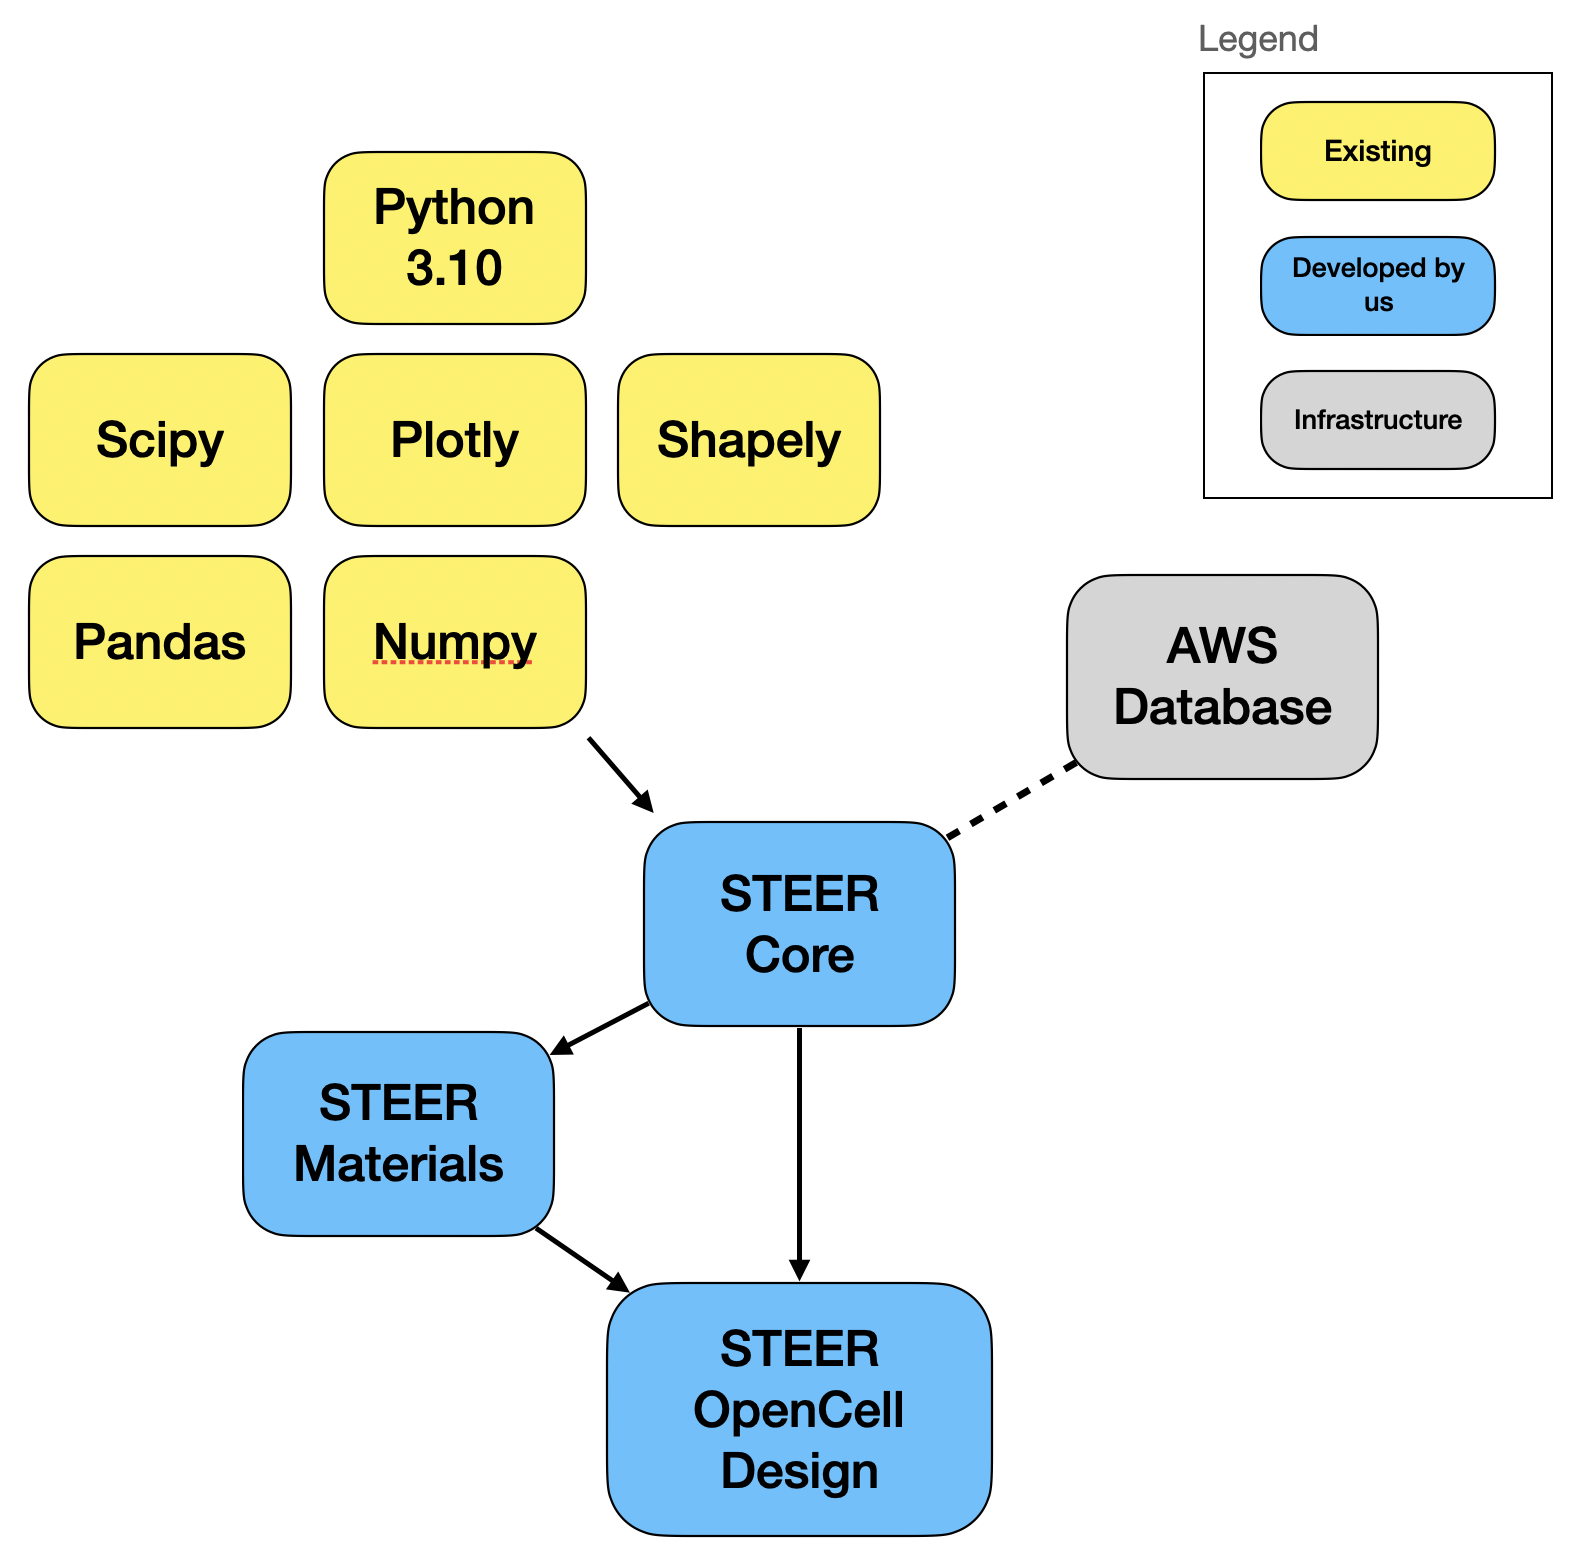
\includegraphics[width=0.55\textwidth]{Figure_1.png}
  \caption{Software dependencies and architecture of OpenCell Design.}
  \label{fig:hierarchy}
\end{figure}

\begin{figure}[tb]
  \centering
  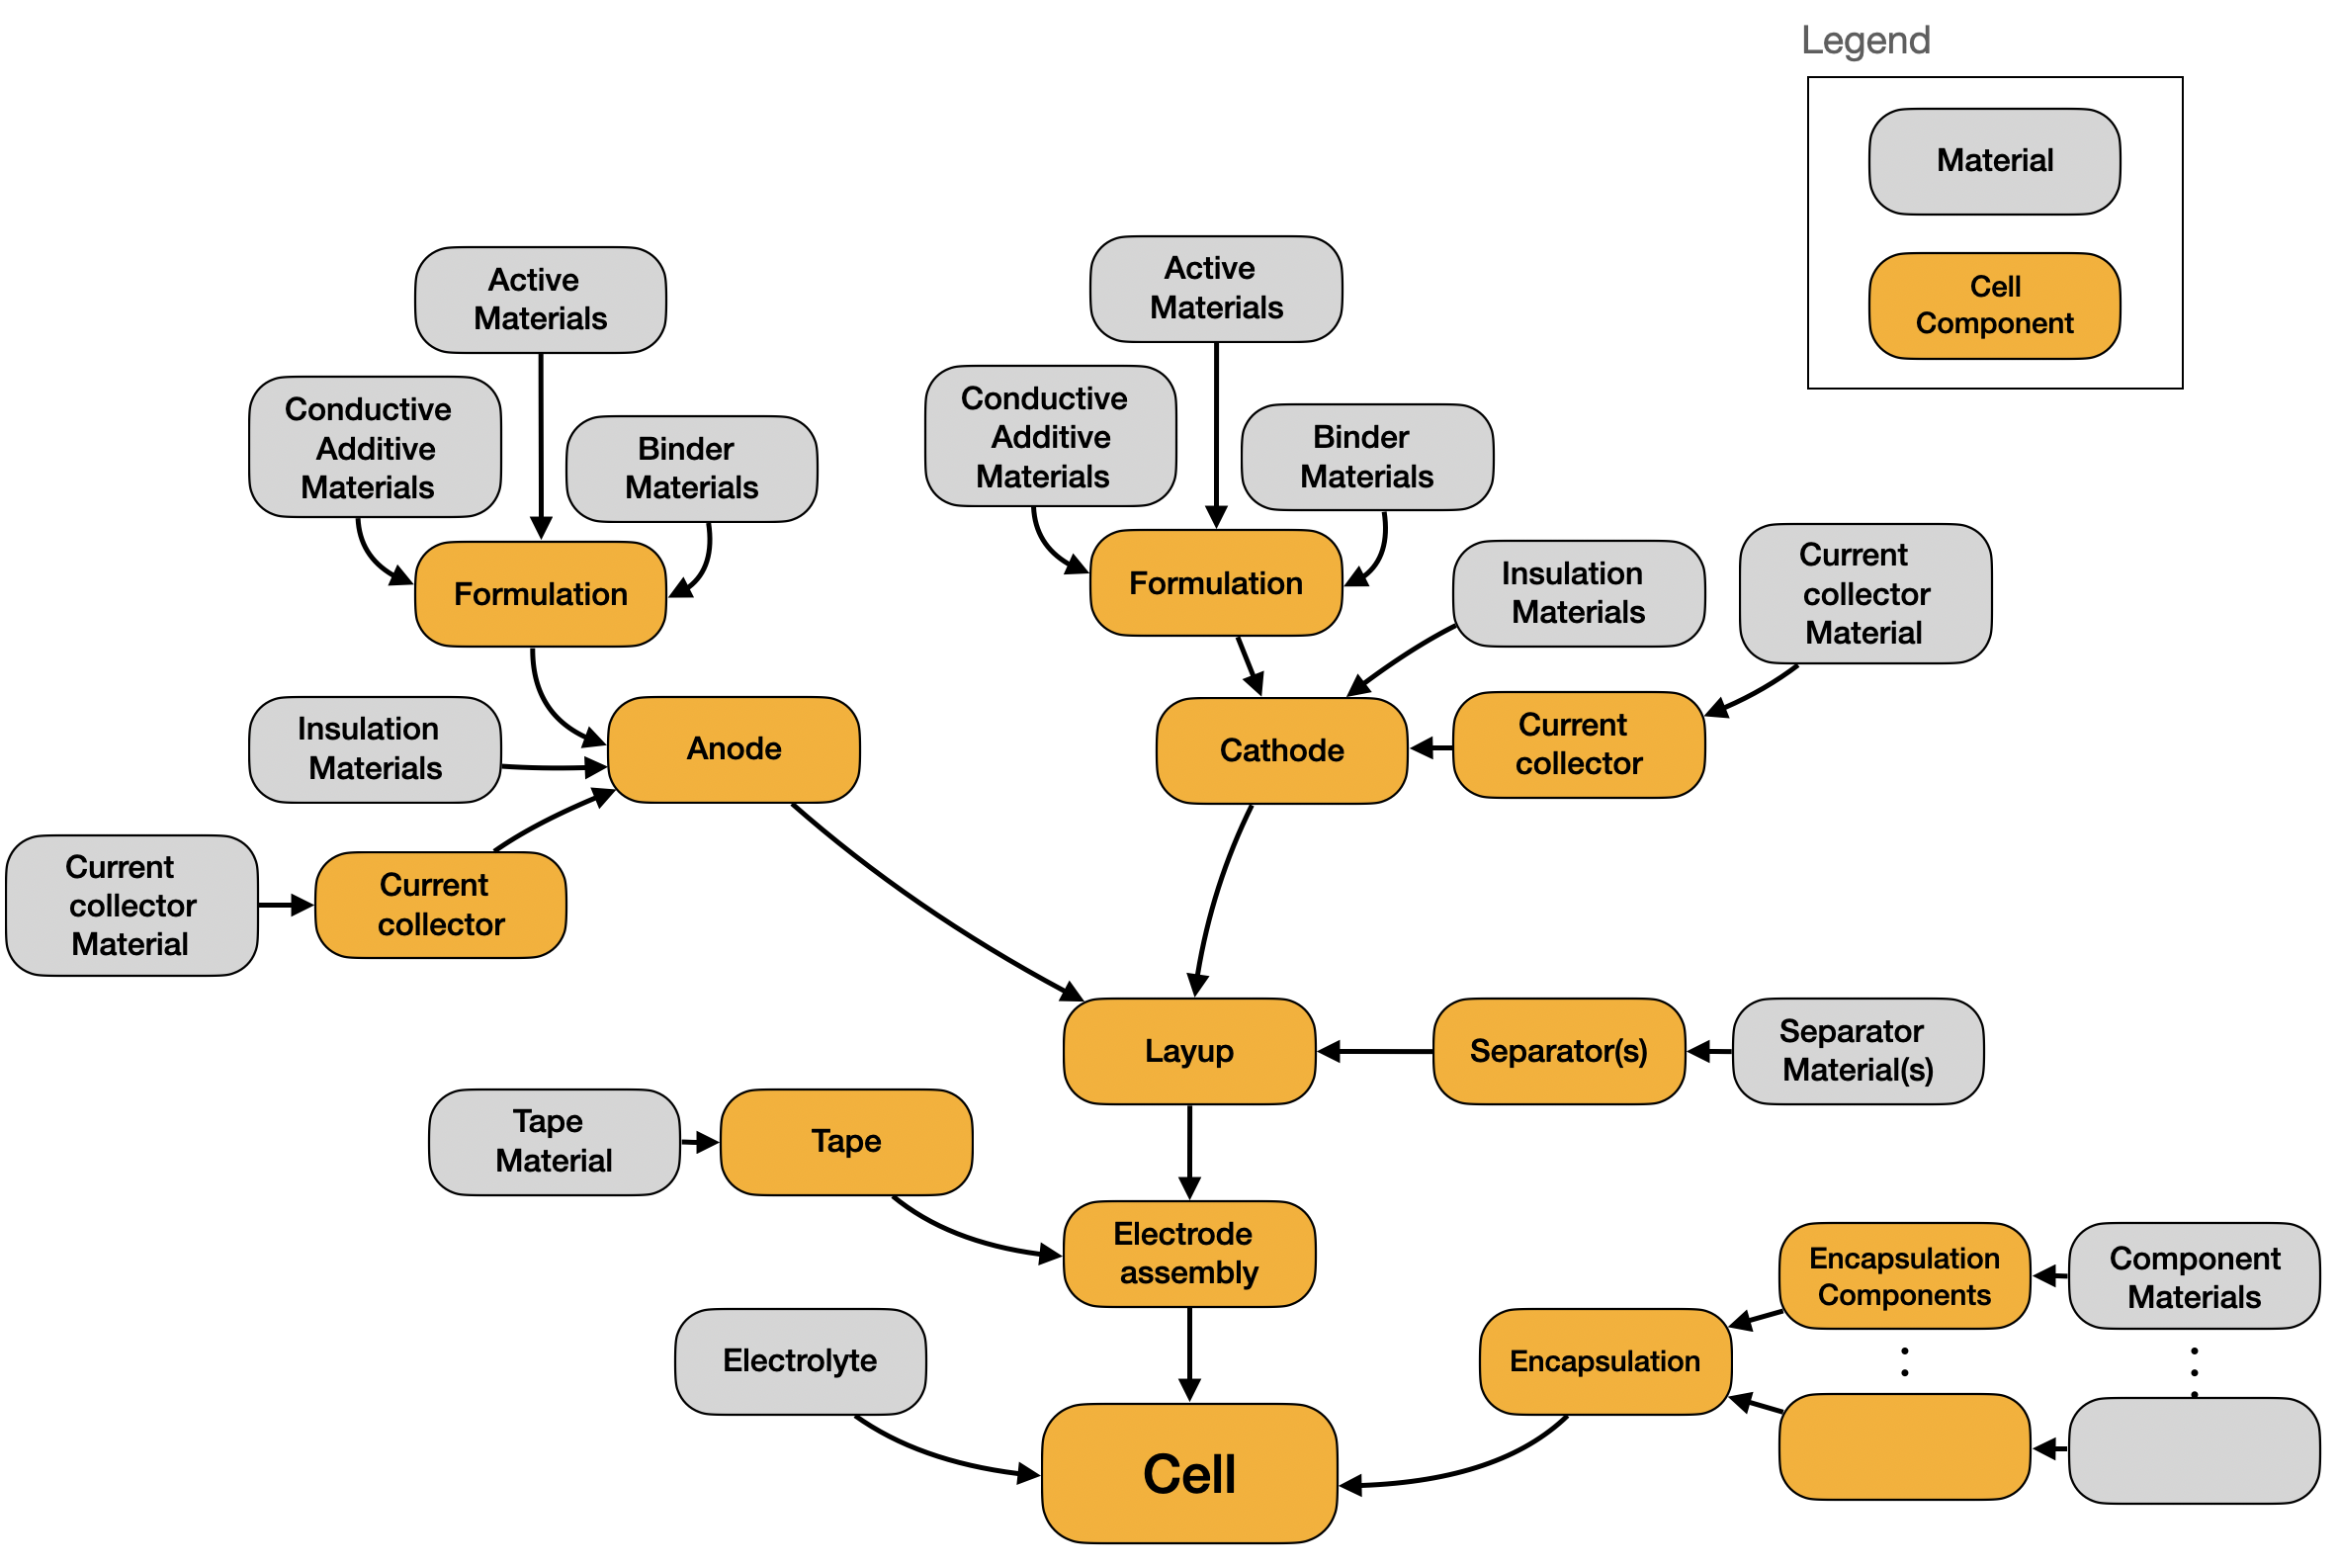
\includegraphics[width=0.85\textwidth]{Figure_2.png}
  \caption{Hierarchical modeling architecture of OpenCell Design, illustrating the composable structure from materials through to complete cells.}
  \label{fig:dependencies}
\end{figure}

OpenCell Design follows these key design principles:

\begin{itemize}[leftmargin=*]
  \item Components are realized through Python classes, enabling a fully object-oriented model.
  \item Components inherit from base classes (Figure~\ref{fig:baseclass} for an example), allowing common logic to exist in the base class and thus allowing new components to be easily defined. Base classes are also implemented as `abstract base classes', enforcing functionality of child classes where needed.
  \item Component classes only contain logic which is relevant to that component. Logic associated with serialization, plotting etc.\ are contained in mixins in \texttt{steer\_core}.
  \item Component attributes are private (with a preceding underscore) and are stored in SI units. They are accessible as `properties', which perform rounding and conversion to user-friendly units.
  \item Attributes are explicitly set using `setters', which perform conversion to SI units, input validation, and carry out logic to keep the model physics-constrained.
  \item Component properties are calculated in the class furthest down the hierarchy tree possible. For example, specific capacity is defined in the active material and formulation components. Areal capacities are defined in the electrode after the formulation has been coated onto the current collector. Capacity is calculated at the cell level, after potentially multiple electrode assemblies may come together.
\end{itemize}

\begin{figure}[tb]
  \centering
  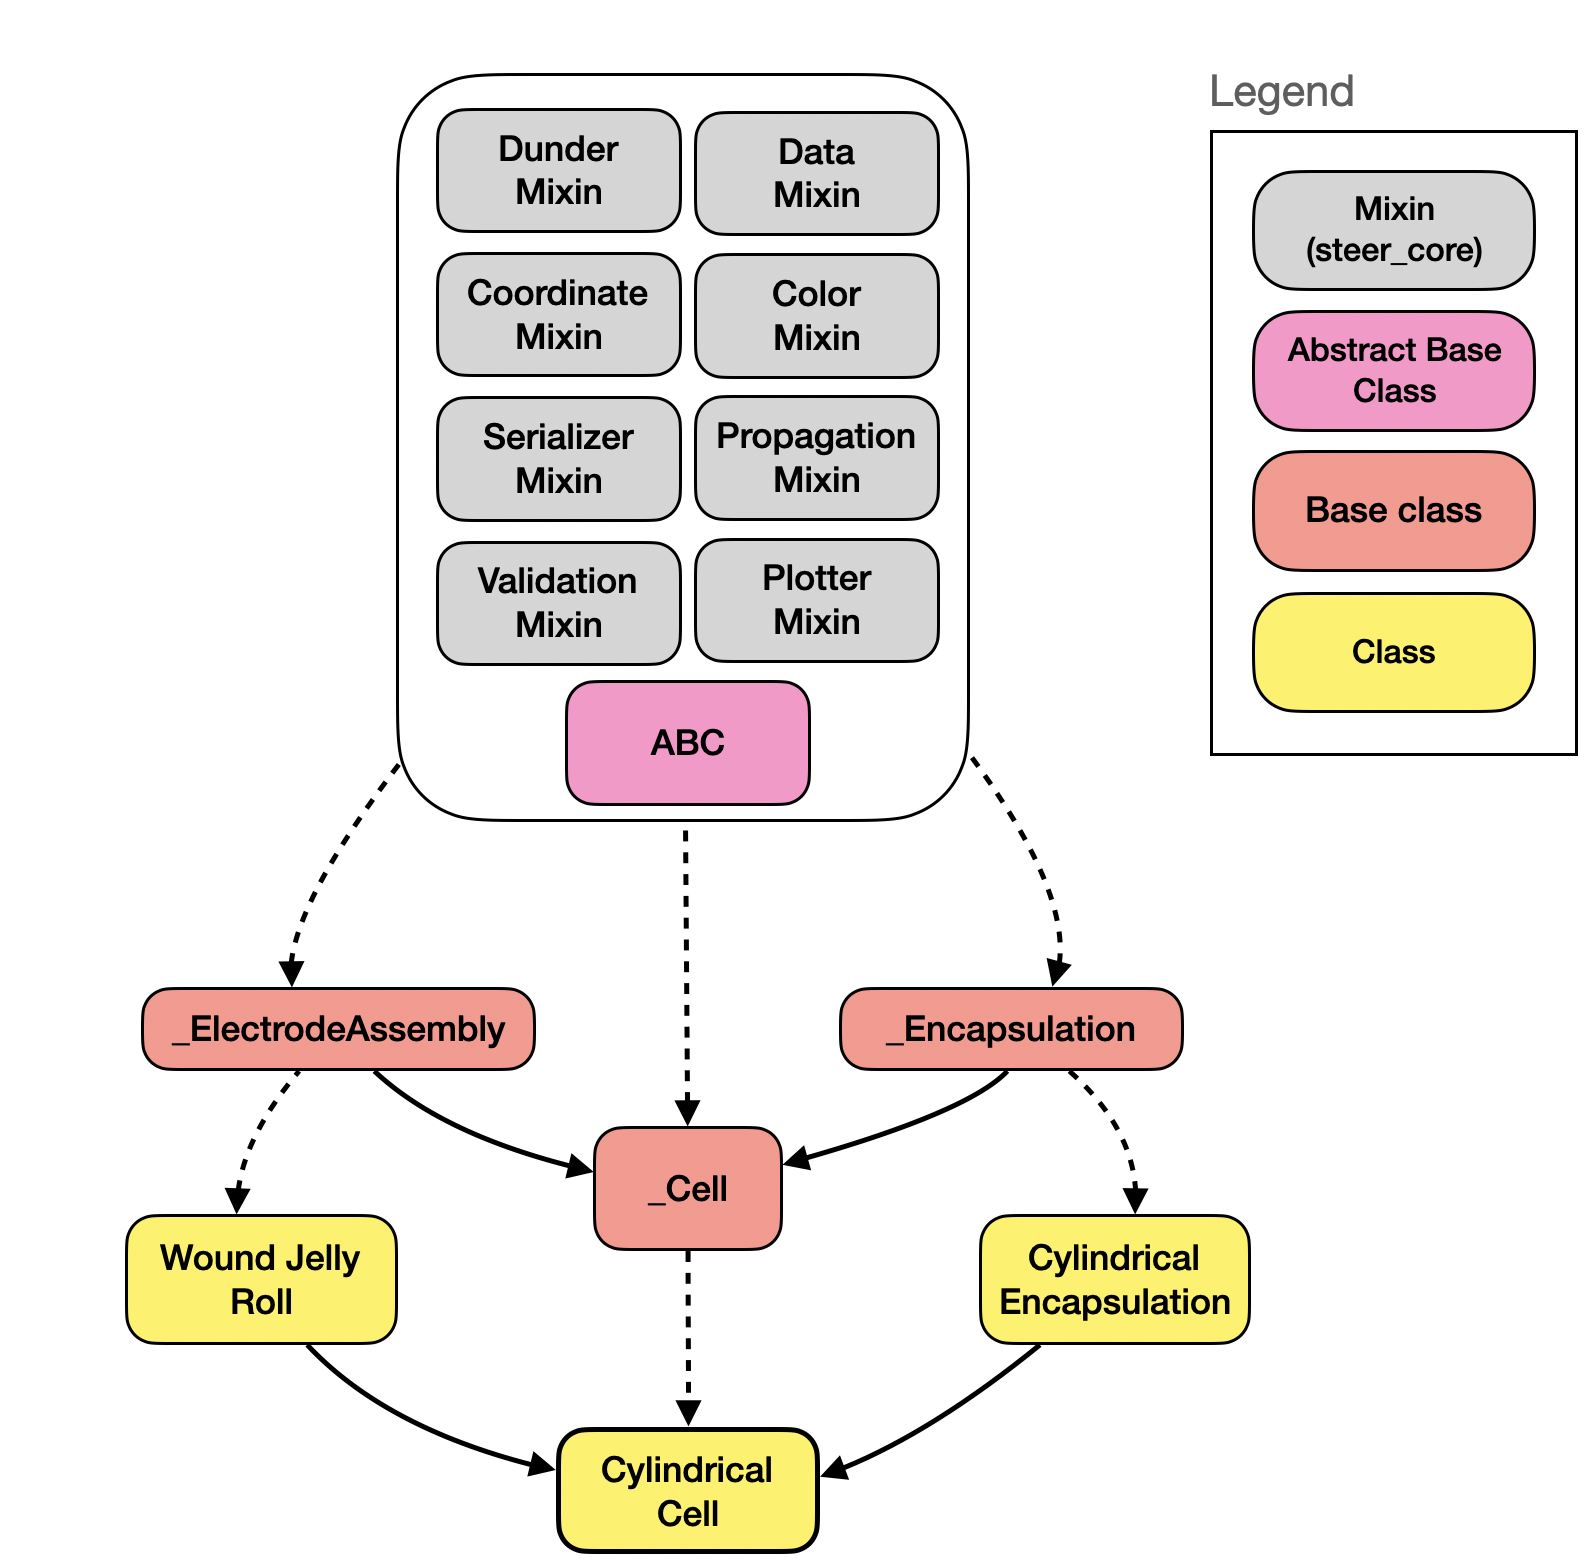
\includegraphics[width=0.65\textwidth]{Figure_3.png}
  \caption{Example base class structure demonstrating the inheritance hierarchy used in OpenCell Design.}
  \label{fig:baseclass}
\end{figure}

The property/setter approach allows for OpenCell Design to be an extensible, bidirectional model. For example, users can modify the n/p ratio of a cell by manipulating the mass loading of the cathode and anode. They can likewise directly set the n/p ratio of the layup, which modifies the cathode and anode mass loading according to a control mode to achieve the desired n/p ratio.

The Pythonic implementation gives access to the many powerful and highly optimized Python libraries for carrying out numerical calculations. Examples include the calculation of thickness-dependent jelly roll spirals via an adaptive RK4 scheme, optimized with a just-in-time compiler~\cite{lam2015numba}, and numerical minima search engines such as the BrentQ algorithm~\cite{brent1971algorithm}, implemented in SciPy~\cite{virtanen2020scipy}.

The object-oriented approach allows for easy extensibility with novel cell types. To demonstrate this, in OpenCell Design we include a class definition for a novel flex-frame cell, representing one of the cell architectures being used to realize solid-state cell technologies. We can fully define the encapsulation in approximately 700 lines of code, and the cell in approximately 300 lines of code, after which the full cell can be modeled through inheriting the cell base classes, and using composition with existing cell components.

%% ============================================================================
\section{Constructing a Cell}
%% ============================================================================

Cell construction follows the hierarchical structure shown in Figure~\ref{fig:hierarchy}. At the materials level, users define active materials, binders, conductive additives, separator materials, current collector materials, and encapsulation materials. Each material is parameterized by density and specific cost. Active materials additionally carry first-cycle half-cell voltage--capacity curves. Alternatively, users can access standard materials using the \texttt{.from\_database()} API for any material class.

Active materials, binders and conductive additives are combined into electrode formulations. Any number of active materials, binders or conductive additives can be added to the formulation. Formulations are then paired with current collectors to create electrodes, with the option to also add electrical insulation strips.

The cathode and anode electrodes are arranged with separators into a layup. For wound cells, a \texttt{Laminate} places the cathode and anode between top and bottom separators; for stacked cells, a \texttt{MonoLayer} uses a single separator between electrode pairs.

The layup is wound or stacked into an electrode assembly. For cylindrical cells, a \texttt{WoundJellyRoll} winds the laminate around a cylindrical mandrel, calculating the number of turns and final outer radius from the layup thickness and mandrel diameter. For prismatic cells, a \texttt{FlatWoundJellyRoll} produces a racetrack-shaped winding with flat sides. For pouch and prismatic cells using stacked configurations, \texttt{ZFoldStack} and \texttt{PunchedStack} assemblies calculate the number of layers required to fill the available volume. The assembly aggregates the total active area, capacity, and mass from the repeated layup units, and adds termination tape for wound designs. Finally, the electrode assembly is combined with an encapsulation and electrolyte to produce the complete cell.

Example scripts on building cells of different formats and internal constructions are included in the supporting information.

%% ============================================================================
\section{Modifying a Cell}
%% ============================================================================

A key challenge in hierarchical cell modeling is maintaining consistency when parameters change. Modifying a property deep in the hierarchy---such as the density of an active material---potentially affects calculations at every level above it: the formulation's blended density, the electrode's coating thickness, the layup's capacity balance, and ultimately the cell's energy and cost. Manually propagating these changes by reassigning objects at each level is tedious and error-prone.

OpenCell Design addresses this through a propagation system that automatically updates dependent calculations when parameters change. Each object in the hierarchy maintains a reference to its parent and knows which attribute it occupies on that parent. When a user modifies a property and calls \texttt{object.propagate\_changes()}, the system triggers the parent's setter by re-assigning the modified object. This invokes the parent's property recalculation logic, which updates all derived quantities at that level. The process then continues upward through the hierarchy until reaching the cell.

For cases requiring finer control, the \texttt{update()} method propagates changes by a single level rather than all the way to the cell. This allows users to modify parameters at intermediate levels between propagation steps, enabling complex design operations that depend on the order of calculations. This level-by-level approach enables studies that would otherwise require rebuilding the cell from scratch, such as comparing designs at constant volume, constant capacity, or constant N/P ratio while varying other parameters.

Examples of using both \texttt{object.propagate\_changes()} and \texttt{object.update()} are included in the supporting information.

%% ============================================================================
\section{Visualizations}
%% ============================================================================

OpenCell Design provides interactive browser-based visualizations using Plotly~\cite{plotly2015}, enabling immediate visual feedback during design iteration. Visualization methods are available at multiple levels of the hierarchy, allowing users to inspect individual components or the complete cell.

Geometric visualizations can show the physical structure of the cell (Figure~\ref{fig:vis}a). Cross-section views display the internal arrangement of electrodes, separators, and current collectors within wound or stacked assemblies---for cylindrical cells, this reveals the spiral structure of the jelly roll; for stacked cells, it shows the layered electrode arrangement. Top-down views display the cell from above, showing tab positions, electrode dimensions, and encapsulation geometry. Side views are available for prismatic and pouch cells to show the stacking arrangement and seal regions.

Electrochemical visualizations display voltage--capacity behavior (Figure~\ref{fig:vis}b). Capacity plots show both charge and discharge curves, with annotations marking the operating voltage window, reversible capacity, irreversible capacity, and capacity loss. These plots update automatically when cell parameters change, providing immediate feedback on how design choices affect electrochemical performance.

\begin{figure}[tb]
  \centering
  \begin{subfigure}[t]{0.38\textwidth}
    \centering
    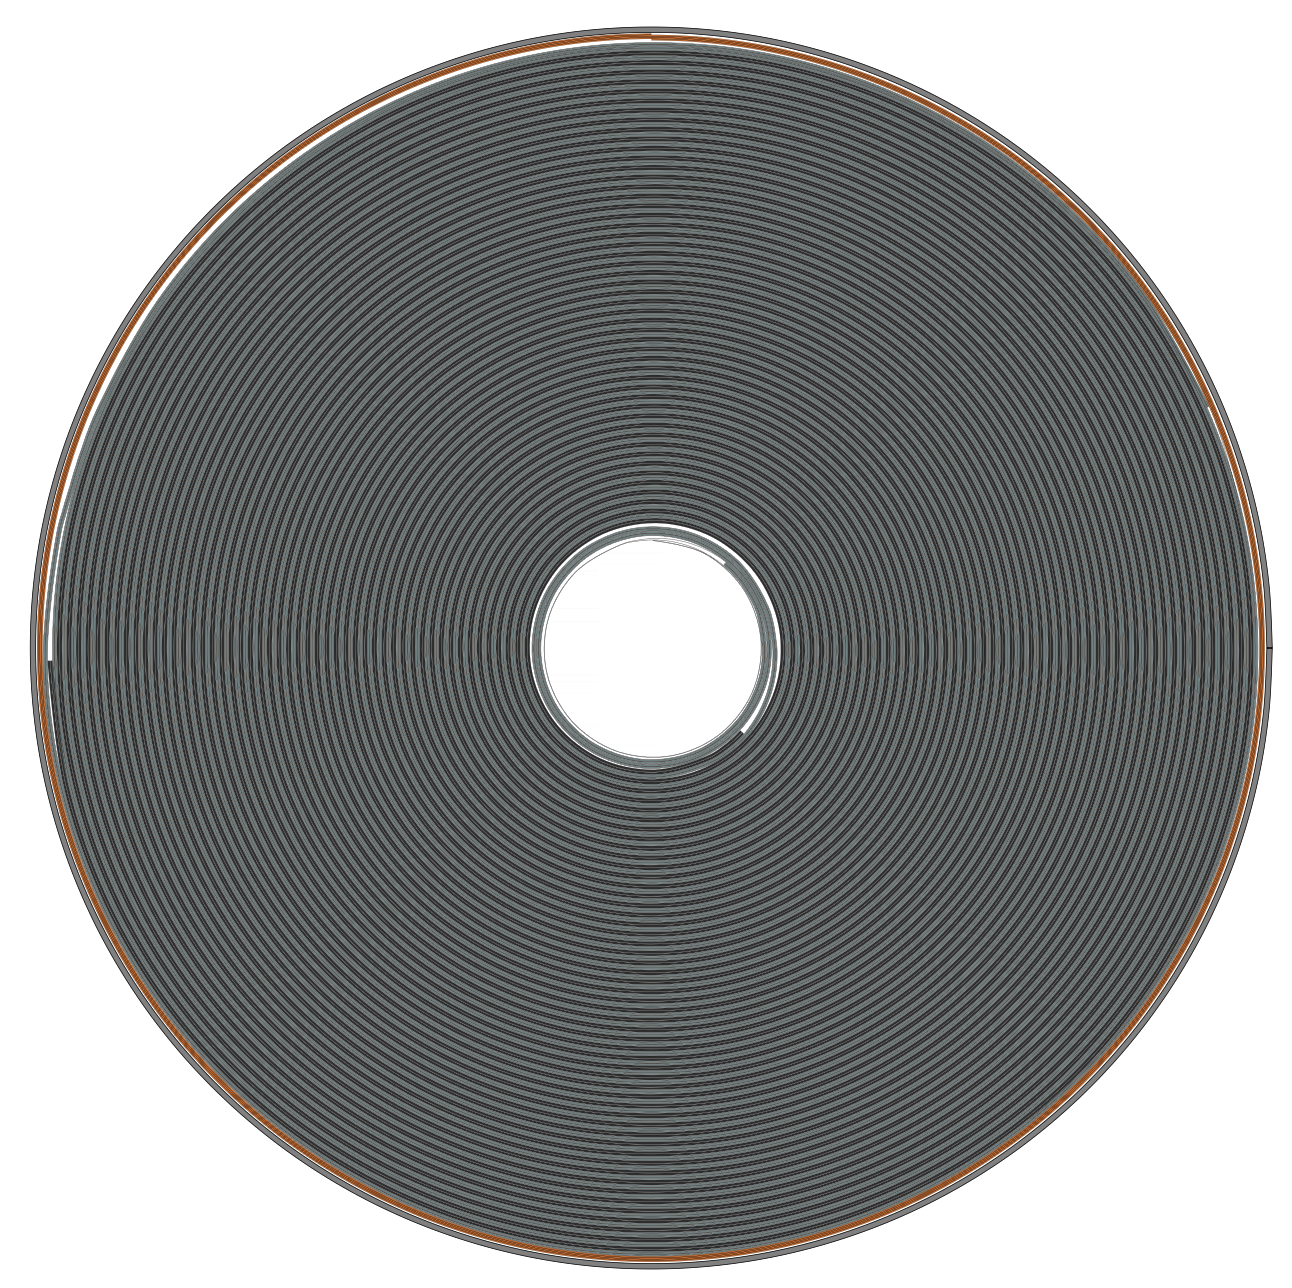
\includegraphics[width=\textwidth]{Figure_4a.png}
    \caption{Cross-section visualization of a cylindrical cell showing the internal arrangement of electrodes, separators, and current collectors.}
    \label{fig:vis_a}
  \end{subfigure}
  \hfill
  \begin{subfigure}[t]{0.58\textwidth}
    \centering
    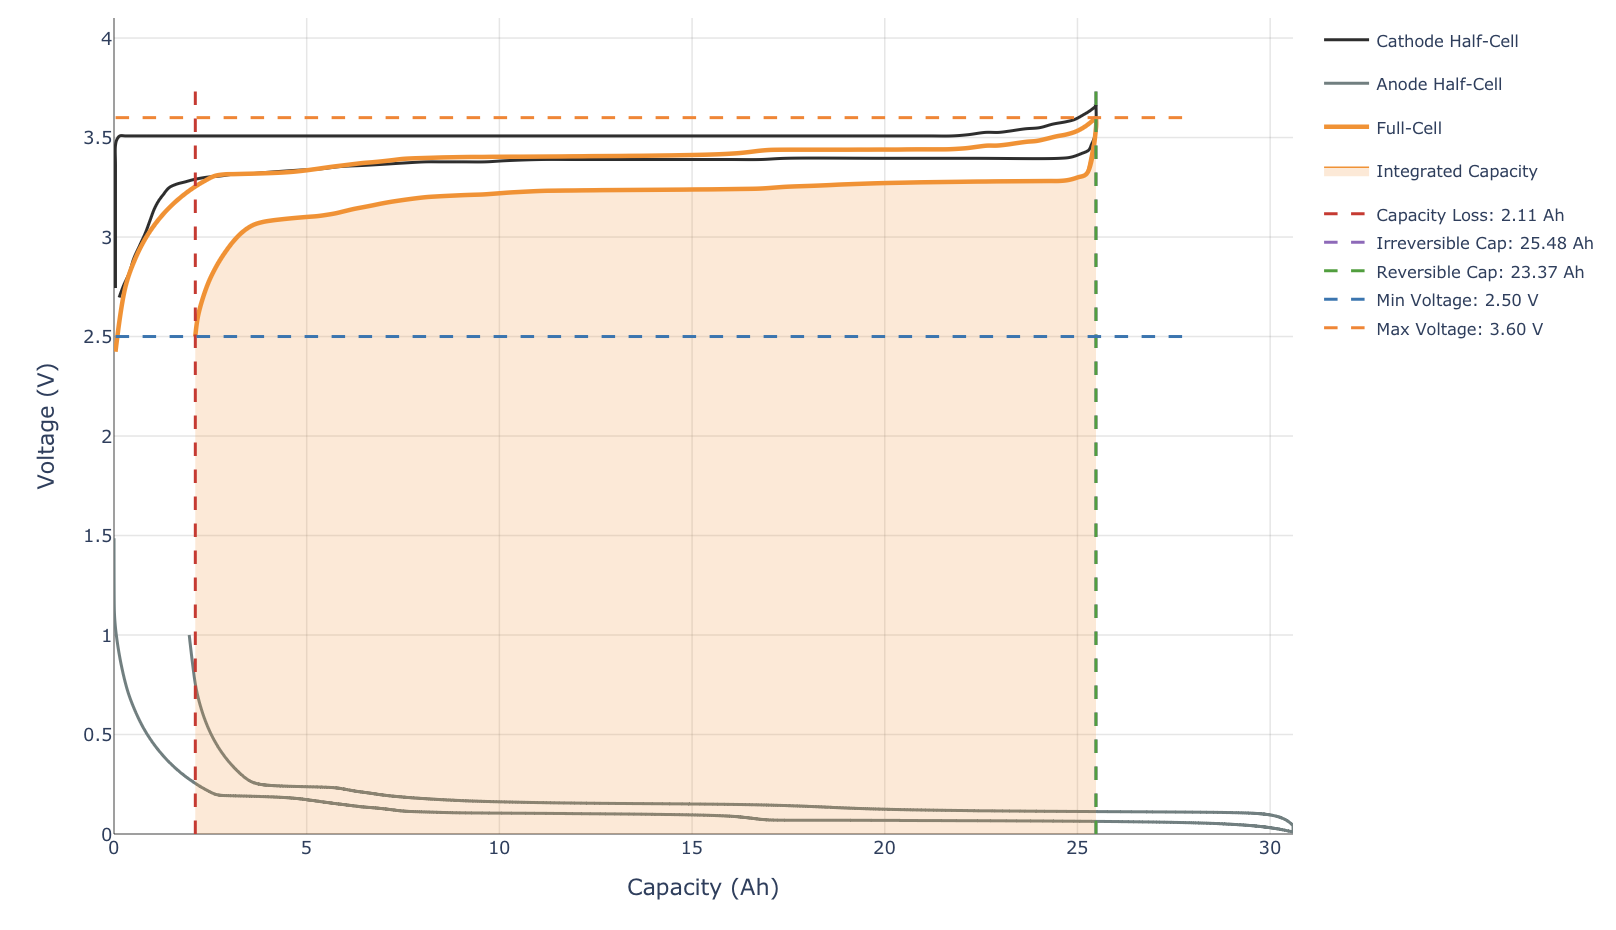
\includegraphics[width=\textwidth]{Figure_4b.png}
    \caption{Voltage--capacity curves showing charge and discharge behavior with annotated capacity metrics.}
    \label{fig:vis_b}
  \end{subfigure}
  \caption{OpenCell Design visualizations: (a) geometric cross-section view and (b) electrochemical voltage--capacity curves.}
  \label{fig:vis}
\end{figure}

Technoeconomic visualizations break down mass and cost contributions using interactive sunburst charts. These hierarchical diagrams show how each component contributes to total cell mass and cost, from raw materials at the innermost ring through to the complete cell at the outermost ring. Users can click to zoom into specific branches of the hierarchy, making it straightforward to identify the dominant cost or mass drivers in a design.

All visualization methods return Plotly figure objects that can be displayed in Jupyter notebooks, saved to image files, or embedded in web applications.

%% ============================================================================
\section{Quality Control}
%% ============================================================================

OpenCell Design includes a comprehensive test suite to ensure correctness and prevent regressions during development. The test suite comprises 12 test modules containing over 700 individual test cases, organized to mirror the package structure: separate modules test materials, formulations, electrodes, current collectors, separators, layups, electrode assemblies, containers, and complete cells.

%% ============================================================================
\section{Conclusion}
%% ============================================================================

OpenCell Design provides an open-source, programmatic framework for designing and analyzing metal-ion battery cells. By implementing a hierarchical modeling architecture that mirrors the physical construction of cells---from raw materials through to complete cell assemblies---OpenCell Design enables users to explore the relationships between material properties, design choices, and cell-level performance and cost metrics.

The propagation system allows rapid design iteration by automatically updating derived quantities when parameters change, eliminating the need to manually rebuild cell models. The modular, object-oriented architecture supports extension with custom materials, current collector geometries, and entirely new cell formats through subclassing. Serialization capabilities enable cell designs to be saved, shared, and version-controlled, while interactive visualizations provide immediate feedback on cell geometry, electrochemical behavior, and cost breakdowns.

The library addresses a gap between electrochemical simulation tools, which focus on physics-based modeling of cell behavior, and spreadsheet-based cost models, which lack extensibility and programmatic access. By providing both capabilities in a composable Python API, OpenCell Design supports workflows ranging from early-stage design exploration to systematic optimization studies. The software is freely available under the GNU Affero General Public License v3.0, with documentation and examples provided in the repository.

%% ============================================================================
%% Bibliography
%% ============================================================================
\bibliographystyle{unsrtnat}
\bibliography{references}

\end{document}
